%!TEX root = ../../thesis.tex

This section describes the \WW cross section measurement using the 
\unit{$\sqrt{s} = 7$}{\TeV} dataset, published in \Reference~\cite{WW-7TeV}.
As the experimental signature is the same as \HWW, many backgrounds are shared.
However, there are two key differences between the analyses. 

\begin{enumerate}
	\item The analysis described in \Chapter~\ref{chap:selection} is optimised for low 
	mass (\unit{$\mH \approx 125$}{\GeV}) resonant \WW production. It therefore requires 
	at least one \PW boson to be off-shell, and consequently employs low lepton 
	thresholds (\unit{$\pt > 10$}{\GeV}). Conversely, the search for non-resonant \WW 
	production is optimised for on-shell \PW bosons, and so raises the lepton thresholds 
	to \unit{$\pt > 20$}{\GeV}. This reduces fake leptons, and obviates the need to split 
	the different flavour channel into \emch and \mech parts.

	\item The total \WW cross section at \unit{$\sqrt{s} = 7$}{\TeV} is 
	\unit{$44.7^{+2.1}_{-1.9}$}{\pico\barn}, which is much larger than that of \ggHWW 
	(\unit{$3.3 \pm 0.4$}{\pico\barn} for \unit{$\mH = 125$}{\GeV}). This enables use of 
	tighter criteria to reduce backgrounds, whilst retaining a large number of signal 
	events. For example, only the 0-jet bin is used.
\end{enumerate}



\subsection{Reconstruction of physics objects}

Beam conditions in 2011 were quite different to 2012; in particular, the pile-up 
environment was much less difficult (see \Figure~\ref{fig:dataset:pileup}). Consequently, 
the reconstruction of physics objects is slightly different to that described in 
\Section~\ref{sec:objects}.

\begin{description}
\item[Electrons] \hfill \\
	The Gaussian Sum Filter was not implemented in the 2011 reconstruction, and so the 
	efficiency is lower (see \Figure~\ref{fig:objects:el_recoeff}). To reduce fakes, the 
	cut-based \textit{tight} identification criteria are used. The reduced pile-up allows
	tighter calorimeter isolation to be applied, $\etcone{0.3}/\et < 0.14$, and this in 
	turn allows for looser tracker isolation $\ptcone{0.3}/\et < 0.13$. Finally, the 
	association with the primary vertex is relaxed, with the transverse impact parameter 
	$d_0$ required to be within ten standard deviations of zero. The threshold is raised 
	to \unit{$\pt > 20$}{\GeV}.

\item[Muons] \hfill \\
	Differences to muon reconstruction are minimal. Slightly tighter quality criteria are 
	applied to the ID tracks. The isolation criteria are $\etcone{0.3}/\pt < 0.14$ and 
	$\ptcone{0.3}/\pt < 0.15$. The threshold is raised to \unit{$\pt > 20$}{\GeV}.

\item[Jets] \hfill \\
	A lower pile-up noise threshold is used in topo-clustering, corresponding to 
	$\mu = 8$. Local cluster weighting (LCW) is not performed on topo-clusters, and so 
	jets are corrected directly from the EM scale to the Jet Energy Scale (JES). In 2011, 
	the pile-up subtraction step of the calibration is less sophisticated, and is 
	averaged over \npv and $\mu$ rather than as an event-by-event correction 
	\cite{Jets:PileupCorrection:2011}. The jet vertex fraction criterion is also removed. 
	Finally, a unified threshold of \unit{$\pt > 25$}{\GeV} is used over the entire 
	range $\mods{\eta} < 4.5$.

\item[Missing transverse momentum] \hfill \\
	Calorimeter-based \met is used exclusively throughout the analysis.

\end{description}



\subsection{Event selection criteria}

As mentioned above, the event selection of the \WW measurement can be tighter than that 
of the \HWW search, and does not require such stringent optimisation.

\begin{description}
\item[Data quality] \hfill \\
	The 2011 \pp dataset (see \Section~\ref{sec:dataset:dataset}) is subject to data 
	quality criteria as in 2012, though some criteria are specific to the data-taking 
	conditions of 2011. The selected dataset corresponds to an integrated luminosity of 
	\unit{$4.64 \pm 0.18$}{\invfb}.

\item[Trigger] \hfill \\
	The lowest unprescaled single lepton triggers were used to support 
	\unit{$\ptleadlep > 25$}{\GeV} in the offline analysis, whilst operating on the 
	plateau. These changed throughout the year as data-taking conditions changed, and 
	are displayed in \Table~\ref{tab:ww:triggers}.

	\begin{table}
		\begin{tabular}{ll@{\hskip 0.3in}r@{\;{--}\;}l}
			\toprule
			\multirow{3}{*}{\Pe}  & \verb|EF_e20_medium|     & 14th Apr & 4th Aug \\
			                      & \verb|EF_e22_medium|     & 4th Aug & 22nd Aug \\
			                      & \verb|EF_e22vh_medium1|  & 7th Sep & 30th Oct \\
			\midrule
			\multirow{2}{*}{\Pmu} & \verb|EF_mu18_MG|        & 14th Apr & 29th Jul \\
			                      & \verb|EF_mu18_MG_medium| & 30th Jul & 30th Oct \\
			\bottomrule
		\end{tabular}
		\caption{Single lepton triggers employed in the 2011 \WW cross section 
		measurement. Trigger names are explained in \Table~\ref{tab:sel:triggers}.}
		\label{tab:ww:triggers}
	\end{table}

\item[Event selection] \hfill \\
	The event selection is shown in \Table~\ref{tab:ww:sel} and is similar to the 0-jet 
	\HWW selection in \Table~\ref{tab:event_selection}, although the topological cuts of 
	the Higgs boson decay are obviously not applied. The major differences are the raised 
	lepton thresholds, the raised \met cuts, and the lack of \dphillmet and \frecoil cuts.

	\begin{table}[b]
		\begin{tabularx}{0.5\textwidth}{YY}
			\toprule
			\emch & \eech/\mmch \\
			\midrule
			\multicolumn{2}{c}{$\ptleadlep > 25$ and $\ptsubleadlep > 20$} \\
			$\mll > 10$    & $\mll > 15$ \\
			--             & $\mods{\mll - \mZ} > 15$ \\
			$\metrel > 25$ & $\metrel > 45$ \\
			\multicolumn{2}{c}{$\njets = 0$} \\
			\multicolumn{2}{c}{$\ptll > 30$} \\
			\bottomrule
		\end{tabularx}
		\caption{Summary of \WW event selection. Cuts are given in \GeV.}
		\label{tab:ww:sel}
	\end{table}

\end{description}



\subsection{Analysis strategy}

In contrast to the \HWW search, the signal region of the \WW measurement has a high 
signal-to-background ratio. Thus, it is sufficient to simply count the number of events 
passing the selection, rather than fit a discriminating observable like \mt.

In order to measure the total \WW cross section, it is necessary to estimate the signal 
acceptance of the event selection (see \Section~\ref{sec:ww:signal}). This extrapolation 
from the measured phase space to the inclusive phase space introduces theoretical 
uncertainties. It is helpful to separate these theoretical uncertainties from the others, 
by measuring an intermediate cross section in a \textit{fiducial region} of phase space, 
chosen to be similar to that used in the detector-level selection in order to minimise 
the extrapolation.

The fiducial region is defined by the criteria in \Table~\ref{tab:ww:sel} applied to 
hadron-level objects, which are now described. The MC event record is used to identify 
leptons and neutrinos which descend from the \PW bosons. An \metvec vector is constructed 
from the neutrinos. Each lepton is `dressed' with the four-momenta of photons within a 
cone of $\Delta R < 0.1$, in order to recover energy lost via QED FSR. Jets are found 
using individual particles as inputs (\cf topo-clusters at detector-level). Muons and 
neutrinos are excluded from jet finding since they interact weakly with the calorimeter. 
Objects must pass the same \pt, $\eta$ and overlap removal criteria applied at 
detector-level.

The fiducial cross section is extracted from measurements using
\begin{equation}
	\sigma_{\WW}^{\text{fid}} = \frac{N_{\text{obs}} - N_{\text{bkg}}}{C_{\WW} \cdot L}
	\label{eq:ww:fid_xs}
\end{equation}
where $N_{\text{obs}}$ is the observed number of events passing the event selection, 
$N_{\text{bkg}}$ is the expected number of background events (see 
\Section~\ref{sec:ww:bkg}), $L$ is the luminosity of the dataset, and $C_{\WW}$ is the 
ratio of the expected number of signal events passing the detector-level selection to 
those passing the fiducial selection. $C_{\WW}$ accounts for detector effects such as 
lepton trigger and reconstruction efficiencies and object mismeasurement due to the 
finite resolution of the detector.

Then the total cross section can be extracted using
\begin{equation}
	\sigma_{\WW} = \frac{N_{\text{obs}} - N_{\text{bkg}}}{C_{\WW} \cdot A_{\WW} \cdot \text{BR} \cdot L}
	\label{eq:ww:total_xs}
\end{equation}
where $A_{\WW}$ is the ratio of the expected number of signal events passing the fiducial 
selection to the total expected number of signal events. $A_{\WW}$ accounts for the 
signal acceptance of the event selection criteria. BR incorporates the branching ratios 
of both \PW bosons for the channel in question, and includes contributions from leptonic 
\Ptau decays.

It is clear from (\ref{eq:ww:fid_xs}) and (\ref{eq:ww:total_xs}) that both signal and 
background modelling are important inputs in measuring a cross section.



\subsection{Signal modelling}
\label{sec:ww:signal}

The \WW process is modelled at NLO by \meps{\mcatnlo}{\fherwig}. The NNLO \ggWW diagrams 
contribute \about3\% to the total cross section, due to the large gluon luminosities at 
the LHC, and are modelled by \meps{\ggtoww}{\fherwig} \cite{gg2ww}. The signal 
acceptances $C_{\WW}$ and $A_{\WW}$ are evaluated using these MC simulations, though 
are corrected for mismodelled trigger and lepton reconstruction efficiencies through 
\textit{in situ} tag-and-probe studies.

The jet veto in the event selection is responsible for the dominant uncertainties in both 
$C_{\WW}$ and $A_{\WW}$. Uncertainties in the jet energy scale (JES) and jet energy 
resolution (JER) lead to large uncertainties in $C_{\WW}$, since the leading jet \pt is a 
rapidly falling distribution. As discussed in \Section~\ref{sec:ggf_jetbin}, restricting 
QCD emissions via a jet veto introduces large theoretical uncertainties to $A_{\WW}$, 
though these are expected to be smaller in \WW than ggF as the perturbative corrections 
are smaller.

For this reason, a data-driven correction factor is included within $C_{\WW}$ in order to 
improve the modelling of the jet veto acceptance $\epsilon_{\WW}$. This correction 
factor is derived using \HepProcess{\PZ \HepTo \Plepton \Plepton} events. Thus, the 
predicted jet veto acceptance is
\begin{equation}
	\epsilon^{\text{pred}}_{\WW} = \epsilon^{\text{MC}}_{\WW} \cdot \frac{\epsilon^{\text{data}}_{\PZ}}{\epsilon^{\text{MC}}_{\PZ}} \,.
\end{equation}
Application of this correction factor effectively calibrates the MC generator to data 
(thus the MC generators used to model $\epsilon^{\text{MC}}_{\WW}$ and 
$\epsilon^{\text{MC}}_{\PZ}$ must be the same). As shown in 
\Table~\ref{tab:ww:jetveto_contrib}, this enables the experimental uncertainty due to the 
jet veto acceptance to be reduced, at the expense of introducing a theoretical 
uncertainty to $C_{\WW}$. However, in the product $C_{\WW} \cdot A_{\WW}$ the 
theoretical uncertainty is also reduced.

Correction factors $\epsilon^{\text{data}}_{\PZ} / \epsilon^{\text{MC}}_{\PZ}$ are 
measured in control regions with high \HepProcess{\PZ \HepTo \Plepton \Plepton} purity. 
Events are selected with \unit{$\ptleadlep > 25$}{\GeV}, \unit{$\ptsubleadlep > 20$}{\GeV}
and \unit{$\mods{\mll - \mZ} < 15$}{\GeV} in the \eech and \mmch channels. The correction 
factor for the \emch channel is taken as the average of the other two. This gave 
correction factors of 0.957, 0.954 and 0.956 for the \eech, \mmch and \emch channels 
respectively. Statistical uncertainties were found to be negligible compared to the 
experimental and theoretical uncertainties.

\begin{table}[b]
	\begin{tabularx}{\textwidth}{c|YY|YY}
		\toprule
		\multirow{2}{*}{Contribution to} & \multicolumn{2}{c|}{No correction factor} & \multicolumn{2}{c}{Jet veto correction factor} \\
		& Exper. & Theor. & Exper. & Theor. \\
		\midrule
		$C_{\WW}$ & $\Delta\epsilon^{\text{MC}}_{\WW}$ & -- & $\Delta\parenths{\epsilon^{\text{MC}}_{\WW} / \epsilon^{\text{MC}}_{\PZ}}$ & $\Delta\epsilon^{\text{MC}}_{\PZ}$ \\
		$A_{\WW}$ & -- & $\Delta\epsilon^{\text{MC}}_{\WW}$ & -- & $\Delta\epsilon^{\text{MC}}_{\WW}$ \\
		$C_{\WW} \cdot A_{\WW}$ & $\Delta\epsilon^{\text{MC}}_{\WW}$ & $\Delta\epsilon^{\text{MC}}_{\WW}$ & $\Delta\parenths{\epsilon^{\text{MC}}_{\WW} / \epsilon^{\text{MC}}_{\PZ}}$ & $\Delta\parenths{\epsilon^{\text{MC}}_{\WW} / \epsilon^{\text{MC}}_{\PZ}}$ \\
		\bottomrule
	\end{tabularx}
	\caption{Summary of how the experimental and theoretical uncertainties on the jet 
	veto acceptance $\epsilon$ contribute to $C_{\WW}$, $A_{\WW}$ and their product. 
	Strategies with and without the jet veto correction factor are considered.}
	\label{tab:ww:jetveto_contrib}
\end{table}

Uncertainties in $\epsilon^{\text{MC}}_{\WW}$ and $\epsilon^{\text{MC}}_{\PZ}$ due to the 
JES are evaluated by increasing and decreasing jet energies by one standard deviation, 
and using the average of the deviations. The JES uncertainty is determined during the 
\textit{in situ} calibration \cite{Jets:Calib:2011}. Similarly, uncertainties due to the 
JER are evaluated by increasing the JER by one standard deviation. The JER uncertainty is 
determined using other \textit{in situ} techniques \cite{Jets:JER:2011}. These 
uncertainties are displayed in \Table~\ref{tab:ww:jetveto_unc}.

Theoretical uncertainties are evaluated at hadron-level by changing some aspect of the MC 
modelling and measuring the effect upon the jet veto acceptance. These uncertainties are 
displayed in \Table~\ref{tab:ww:jetveto_unc}, and their estimation is described below.

\begin{table}
	\begin{tabular}{r|ccccc|cc}
		\toprule
		& \multicolumn{5}{c|}{Uncertainty sources} & \multicolumn{2}{c}{Total} \\
		& JES & JER & Scale & PDF & PS/UE & Exper. & Theor. \\
		\midrule
		\multicolumn{8}{c}{\emch channel} \\
		\midrule
		$\epsilon^{\text{MC}}_{\WW} = 0.662$ 
		& 4.6\% & 2.4\% & 5.3\% & 1.6\% & 0.5\% & 5.1\% & 5.6\% \\
		$\epsilon^{\text{MC}}_{\PZ} = 0.793$ 
		& 3.8\% & 2.6\% & 2.4\% & 0.8\% & 0.4\% & 4.6\% & 2.6\% \\
		$\epsilon^{\text{MC}}_{\WW} / \epsilon^{\text{MC}}_{\PZ} = 0.835$ 
		& 0.7\% & 0.2\% & 3.4\% & 0.9\% & 0.1\% & 0.7\% & 3.5\% \\
		\midrule
		\multicolumn{8}{c}{\eech channel} \\
		\midrule
		$\epsilon^{\text{MC}}_{\WW} = 0.652$ 
		& 4.8\% & 2.0\% & 5.3\% & 1.6\% & 0.5\% & 5.2\% & 5.6\% \\
		$\epsilon^{\text{MC}}_{\PZ} = 0.798$ 
		& 3.7\% & 2.4\% & 2.4\% & 0.8\% & 0.4\% & 4.4\% & 2.6\% \\
		$\epsilon^{\text{MC}}_{\WW} / \epsilon^{\text{MC}}_{\PZ} = 0.817$ 
		& 1.1\% & 0.4\% & 3.4\% & 0.9\% & 0.1\% & 1.2\% & 3.5\% \\
		\midrule
		\multicolumn{8}{c}{\mmch channel} \\
		\midrule
		$\epsilon^{\text{MC}}_{\WW} = 0.655$ 
		& 4.8\% & 2.1\% & 5.3\% & 1.6\% & 0.5\% & 5.2\% & 5.6\% \\
		$\epsilon^{\text{MC}}_{\PZ} = 0.788$ 
		& 4.0\% & 2.8\% & 2.4\% & 0.8\% & 0.4\% & 4.9\% & 2.6\% \\
		$\epsilon^{\text{MC}}_{\WW} / \epsilon^{\text{MC}}_{\PZ} = 0.831$ 
		& 0.8\% & 0.7\% & 3.4\% & 0.9\% & 0.1\% & 1.0\% & 3.5\% \\
		\bottomrule
	\end{tabular}
	\caption{Relative uncertainties in the \WW and \PZ jet veto acceptances, and in their 
	ratio. Results for the \eech, \mmch and \emch channels are shown separately, with 
	$\epsilon^{\text{MC}}_{\PZ}$ for the \emch channel taken as average of the other two.}
	\label{tab:ww:jetveto_unc}
\end{table}

Uncertainties due to higher order corrections are evaluated using the combined inclusive 
method described in \Section~\ref{sec:ggF:ci}. The renormalisation and factorisation 
scales are independently varied in the range $\mu_0/2 \leq \mur,\muf \leq 2\mu_0$, where 
$\mu_0$ is the default scale for the process in question\footnote{
	The default scales used by \mcatnlo are determined by 
	$\mu_0^2 = m_{\Plepton\Plepton}^2 + p_{\text{T,\HepProcess{\Plepton\Plepton}}}^2$ 
	for \PZ production and 
	$\mu_0^2 = (m_{\Plepton\Pnu}^2 + p_{\text{T,\HepProcess{\Plepton\Pnu}}}^2 + 
	m_{\Plepton'\Pnu'}^2 + p_{\text{T,\HepProcess{\Plepton'\Pnu'}}}^2) / 2$
	for \WW production.
}, whilst observing the constraint $1/2 \leq \mur/\muf \leq 2$. The largest deviation is 
used as the uncertainty.

Uncertainties due to \acp{PDF} are evaluated in two ways. The jet veto acceptance 
predicted with the CT10 PDF is compared to that predicted with the MSTW2008 PDF 
\cite{MSTW}. Also, the set of PDF eigenvectors corresponding to 90\% \ac{CL} of the CT10 
fit were used to evaluate an uncertainty.

Uncertainties due to the \ac{PS}, hadronisation and \ac{UE} models are evaluated by 
recomputing the jet veto acceptances with \powhegbox events, and comparing the result 
when showered by \fherwig and \pythia{6}.

By substituting uncertainties from \Table~\ref{tab:ww:jetveto_unc} into the two 
strategies outlined in \Table~\ref{tab:ww:jetveto_contrib}, it is clear that the jet veto 
correction factor offers a significant reduction in uncertainty. Considering the 
$\sigma_{\WW}$ extraction from the \emch channel, the contribution of the experimental 
uncertainty in $\epsilon_{\WW}$ reduces from 5.1\% to 0.7\%, while the theoretical 
uncertainty reduces from 5.6\% to 3.5\%. However, it does introduce a theoretical 
uncertainty to $\sigma^{\text{fid}}_{\WW}$ of 2.6\%.

The signal acceptances $A_{\WW}$, $C_{\WW}$ and $C_{\WW} \cdot A_{\WW}$ are displayed in 
\Table~\ref{tab:ww:cww_aww}. The \mmch channel has the best reconstruction efficiency and 
the event selection of the \emch channel has the highest yield. The uncertainties arising 
from different systematic sources are also shown, with those associated with the jet veto 
separated for clarity. For simplicity, the JES/JER uncertainty in the jet veto acceptance 
are treated as uncorrelated with those of the other cuts. The same is true of the 
theoretical uncertainties in $A_{\WW}$. 

\begin{table}
	\begin{tabular}{l@{}c@{\hskip 0.2in}c@{\hskip 0.2in}c@{\hskip 0.2in}c}
		\toprule
		& \emch & \eech & \mmch & All \\
		\midrule
		$C_{\WW}$ ($\times 100$) & $50.5\pm1.6$ & $40.3\pm1.7$ & $68.7\pm2.1$ & $52.0\pm1.7$ \\
		\quad Trigger efficiency & 0.3\% & 0.1\% & 0.6\% & 0.4\% \\
		\quad Lepton efficiency  & 1.4\% & 2.9\% & 0.7\% & 1.3\% \\
		\quad Lepton \pt scale and resolution & 0.6\% & 0.9\% & 0.8\% & 0.5\% \\
		\quad Jet energy scale and resolution \\
		\quad\quad Jet veto      & 0.7\% & 1.2\% & 1.0\% & 1.0\% \\
		\quad\quad Other cuts    & 0.5\% & 0.6\% & 0.5\% & 0.5\% \\
		\quad \met modelling     & 0.4\% & 0.5\% & 0.2\% & 0.2\% \\
		\quad PDFs, \mur and \muf scales \\
		\quad\quad Acceptance    & 0.3\% & 0.7\% & 0.7\% & 0.3\% \\
		\quad\quad Jet veto correction factor & 2.6\% & 2.6\% & 2.6\% & 2.6\% \\
		\cmidrule(lr){1-5}
		$A_{\WW}$ ($\times 100$) & $15.9\pm0.9$ & $7.5\pm0.4$ & $8.1\pm0.5$ & $11.9\pm0.7$ \\
		\quad PDFs, \mur and \muf scales \\
		\quad\quad Jet veto   & 5.6\% & 5.6\% & 5.6\% & 5.6\% \\
		\quad\quad Other cuts & 1.1\% & 1.0\% & 1.0\% & 1.0\% \\
		\cmidrule(lr){1-5}
		$C_{\WW} \cdot A_{\WW}$ ($\times 100$) & $8.03\pm0.33$ & $3.02\pm0.15$ & $5.56\pm0.22$ & $6.19\pm0.25$ \\
		\quad PDFs, \mur and \muf scales \\
		\quad\quad Jet veto   & 3.5\% & 3.5\% & 3.5\% & 3.5\% \\
		\bottomrule
	\end{tabular}
	\caption{The signal acceptances $C_{\WW}$, $A_{\WW}$ and $C_{\WW} \cdot A_{\WW}$. 
	A breakdown of the relative uncertainties from different sources is also shown. The 
	contribution to $\Delta \parenths{C_{\WW} \cdot A_{\WW}}$ of the theoretical 
	uncertainty in the jet veto is also stated, in order to explicitly exhibit the 
	cancellations between $\Delta C_{\WW}$ and $\Delta A_{\WW}$.}
	\label{tab:ww:cww_aww}
\end{table}



\subsection{Background modelling}
\label{sec:ww:bkg}

The background estimation techniques of the \HWW search are more sophisticated than those 
of the \WW measurement at \unit{$\sqrt{s} = 7$}{\TeV}. For this reason, the techniques 
used in the \WW measurement are only described briefly here, whereas those of the \HWW 
search shall be discussed in detail in \Section~\ref{sec:ww_as_bkg} and 
\Chapter~\ref{chap:backgrounds}.

Although many backgrounds are modelled by a data-driven technique, there is often some 
underlying dependence upon MC. For this reason, \Table~\ref{tab:ww:mc_samples} states the 
MC generators used to model each process.

\begin{table}
	\begin{tabular}{c@{\hskip 0.3in}c}
		\toprule
		Process & MC generator \\
		\midrule
		\ttbar               & \meps{\mcatnlo}{\fherwig} \\
		single top           & \meps{\acermc}{\pythia{6}} \\
		\Wjets, \DY, \Wgamma & \meps{\alpgen}{\fherwig} \\
		\Wgstar              & \meps{\madgraph}{\pythia{6}} \\
		\WZ, \ZZ             & \fherwig \\
		\bottomrule
	\end{tabular}
	\caption{MC generators used to model backgrounds to the \WW measurement.}
	\label{tab:ww:mc_samples}
\end{table}

\begin{description}
\item[\Wjets and dijet] \hfill \\
	The \Wjets background comprises events where a jet is misidentified as a lepton. The 
	fake rate is poorly modelled by MC, and so a data-driven \textit{fake factor method} 
	is used. The dijet background, where two jets fake leptons, is very small and is 
	simultaneously estimated by this method.

	A \Wjets anti-ID region (AR) is defined similarly to the signal region (SR), but 
	where one of the leptons is replaced with an anti-identified lepton. The anti-ID 
	lepton objects are ensured to be highly contaminated with jets by loosening the 
	selection criteria and vetoing leptons passing the full identification. Anti-ID 
	electrons have looser calorimeter isolation criteria and do not have to pass the 
	\textit{tight} identification criteria. Anti-ID muons have looser calorimeter 
	isolation criteria and the tracker isolation removed completely. The predicted \Wjets 
	background is the measured number of events in the AR, scaled by a fake factor 
	$f_{\Plepton}$:
	\begin{equation}
		N_{\text{\Wjets}}^{\text{pred,SR,\HepProcess{\Pe\Pe}}} &= f_{\Pe} \cdot N^{\text{data,AR}}_{\text{id \Pe + anti-id \Pe}} \\
		N_{\text{\Wjets}}^{\text{pred,SR,\HepProcess{\Pmu\Pmu}}} &= f_{\Pmu} \cdot N^{\text{data,AR}}_{\text{id \Pmu + anti-id \Pmu}} \\
		N_{\text{\Wjets}}^{\text{pred,SR,\HepProcess{\Pe\Pmu}}} &= f_{\Pe} \cdot N^{\text{data,AR}}_{\text{id \Pmu + anti-id \Pe}} + f_{\Pmu} \cdot N^{\text{data,AR}}_{\text{id \Pe + anti-id \Pmu}} \,.
	\end{equation}
	The fake factor $f_{\Plepton}$ is defined as the ratio of efficiencies for jets 
	passing the lepton ID criteria to passing the anti-ID criteria ($f_{\Pe} \ll f_{\Pmu}$
	since the electron anti-ID accepts more jets). Each fake factor is measured from 
	dijet events as a function of \pt and $\eta$
	\begin{equation}
		f_{\Plepton} = \frac{N_{\text{id \Plepton}}^{\text{data}}}{N_{\text{anti-id \Plepton}}^{\text{data}}} \,.
	\end{equation}
	To avoid bias, the dijet events were selected with a very loose (but prescaled) 
	trigger, without identification or isolation criteria applied. A \PZ veto 
	(\unit{$\mods{\mll - \mZ} > 15$}{\GeV}) and a \PW veto (\unit{$\mt > 30$}{\GeV}) 
	reject most of the true leptons, and residual electroweak contamination is subtracted 
	using MC.

	The dominant source of uncertainty stems from the fact that the fake factor is 
	derived from dijet events but applied to \Wjets events. This process dependence is 
	estimated with MC. It would be preferable to measure the fake factor from \Zjets 
	events, though this was statistically limited in the \unit{$\sqrt{s} = 7$}{\TeV} 
	dataset. This point shall be revisited in \Section~\ref{sec:wjets} when considering 
	the \Wjets background to the \HWW search.

\item[Top] \hfill \\
	The jet veto is effective at rejecting the top background. The number of surviving 
	top events are estimated by a data-driven \textit{template method}, which attempts to 
	constrain the jet multiplicity distribution within a top control region (CR).

	An inclusive signal region (ISR) is defined without the jet veto and \ptll cut. The 
	top CR is a subset of the ISR, requiring at least one \Pbottom-tagged jet with 
	\unit{$\pt > 20$}{\GeV}. The \njets distribution $\mathcal{T}$ is measured in the CR, 
	and is extrapolated to the ISR by top MC. However, non-top contributions to the CR 
	must be subtracted beforehand, which are estimated by an \njets template from MC 
	scaled by a data-driven normalisation factor $K_{\text{non-top}}^{\text{data}}$. 
	Thus, the predicted top \njets distribution in the ISR is
	\begin{equation}
		\mathcal{T}_{\text{top}}^{\text{pred,ISR}} = \frac{\mathcal{T}_{\text{top}}^{\text{MC,ISR}}}{\mathcal{T}_{\text{top}}^{\text{MC,CR}}} \parenths{\mathcal{T}^{\text{data,CR}} - K_{\text{non-top}}^{\text{data}} \cdot \mathcal{T}_{\text{non-top}}^{\text{MC,CR}}} \,.
	\end{equation}
	$K_{\text{non-top}}^{\text{data}}$ is assumed to be the same in the CR and the ISR, 
	and is constrained by an \njets fit in the ISR, \ie
	\begin{equation}
		\mathcal{T}^{\text{data,ISR}} = \mathcal{T}_{\text{top}}^{\text{pred,ISR}} + K_{\text{non-top}}^{\text{data}} \cdot \mathcal{T}_{\text{non-top}}^{\text{MC,ISR}} \,.
	\end{equation}
	The fit yields $K_{\text{non-top}}^{\text{data}} = 1.07 \pm 0.03$.
	Finally, once the 0-jet bin of $\mathcal{T}_{\text{top}}^{\text{pred,ISR}}$ is 
	selected, the acceptance of the \ptll cut is modelled by top MC.

	The small number of 0-jet events in the top CR leads to a large statistical 
	uncertainty in this background. The systematic uncertainty is dominated by 
	uncertainties in the (mis)tag efficiency of the \Pbottom-tagging algorithm.

\item[\DY] \hfill \\
	The \DY background is suppressed by the \PZ mass veto and the \met and \ptll cuts, 
	though remains a significant background to the \eech and \mmch channels. Since MC 
	might mismodel the fake \met distribution, this background is normalised to data in a 
	control region (CR) that includes the \met cut.

	The \DY CR is defined similarly to the signal region (SR), with the \ptll cut 
	inverted. The number of events in the CR is measured, the non-\DY contamination is 
	subtracted via MC, and the result is extrapolated to the SR using MC:
	\begin{equation}
		N_{\text{\DY}}^{\text{pred,SR}} = \frac{N_{\text{\DY}}^{\text{MC,SR}}}{N_{\text{\DY}}^{\text{MC,CR}}} \parenths{N_{\text{\DY}}^{\text{data,CR}} - N_{\text{non-\DY}}^{\text{MC,CR}}} \,.
	\end{equation}

	The dominant uncertainties are due to the small number of events in the CR and the 
	energy scale of the soft terms in the \met (see \Section~\ref{sec:objects:met}).

\item[Non-\WW diboson] \hfill \\
	The non-\WW diboson backgrounds (\WZ, \Wgstar, \ZZ, \Wgamma) are estimated purely 
	from MC simulation (see \Table~\ref{tab:ww:mc_samples}). The cross section of each 
	process is calculated at NLO with \mcfm.  The dominant uncertainties are theoretical 
	uncertainties in the cross section and JES uncertainties in the jet veto.

\end{description}



\subsection{Experimental results}
\label{sec:ww:results}

The observed number of events passing the event selection is shown for each channel in 
\Table~\ref{tab:ww:sr_yield}. The expected number of events is also shown, with the 
signal and background contributions estimated as described in 
Sections~\ref{sec:ww:signal} and \ref{sec:ww:bkg}, respectively. Systematic uncertainties 
of the \DY and non-\WW diboson backgrounds are considered correlated, though those of the 
other backgrounds are considered uncorrelated. An initial glance suggests that the 
measured cross section shall be higher than predicted. Two different \pt distributions of 
the selected events are displayed in \Figure~\ref{fig:ww:sr_distributions}.

\begin{table}
	\begin{tabular}{l@{\hskip 0.2in}r@{$\,\pm\,$}r@{$\,\pm\,$}r@{\hskip 0.2in}r@{$\,\pm\,$}r@{$\,\pm\,$}r@{\hskip 0.2in}r@{$\,\pm\,$}r@{$\,\pm\,$}r@{\hskip 0.2in}r@{$\,\pm\,$}r@{$\,\pm\,$}l}
		\toprule
		& \multicolumn{3}{c@{\hskip 0.2in}}{\emch} & \multicolumn{3}{c@{\hskip 0.2in}}{\eech} & \multicolumn{3}{c@{\hskip 0.2in}}{\mmch} & \multicolumn{3}{c}{All} \\
		\midrule
		Observed & \multicolumn{1}{c@{\phantom{$\,\pm\,$}}}{821} & \multicolumn{1}{c}{} && \multicolumn{1}{c@{\phantom{$\,\pm\,$}}}{174} & \multicolumn{1}{c}{} && \multicolumn{1}{c@{\phantom{$\,\pm\,$}}}{330} & \multicolumn{1}{c}{} && \multicolumn{1}{c@{\phantom{$\,\pm\,$}}}{1325} \\
		Expected           & 744 & 24 & 57  &  169 & 12 & 16  &  280 & 16 & 20  &  1192 & 31 & 87 \\
		\cmidrule(lr){1-13}
		\quad \WW          & 538 &  3 & 45  &  100 &  2 &  9  &  186 &  2 & 15  &   824 &  4 & 69 \\
		\quad Background   & 206 & 24 & 35  &   68 & 12 & 13  &   94 & 15 & 13  &   369 & 31 & 53 \\
		\cmidrule(lr){1-13}
		\quad\quad Top     &  87 & 23 & 13  &   22 & 12 &  3  &   32 & 14 &  5  &   141 & 30 & 22 \\
		\quad\quad \Wjets  &  70 &  2 & 31  &   21 &  1 & 11  &    7 &  1 &  3  &    98 &  2 & 43 \\
		\quad\quad \DY     &   5 &  2 &  1  &   12 &  3 &  3  &   34 &  6 & 10  &    51 &  7 & 12 \\
		\quad\quad Diboson &  44 &  2 &  6  &   13 &  1 &  2  &   21 &  1 &  2  &    78 &  2 & 10 \\
		\bottomrule
	\end{tabular}
	\caption{The number of events observed and expected in the \unit{4.6}{\invfb} dataset 
	in each signal region. A breakdown of the expected signal and background 
	contributions is also shown, with statistical and systematic uncertainties. The \WW 
	signal is normalised to the NLO cross section of \unit{44.7}{\pico\barn}.}
	\label{tab:ww:sr_yield}
\end{table}

\begin{figure}
	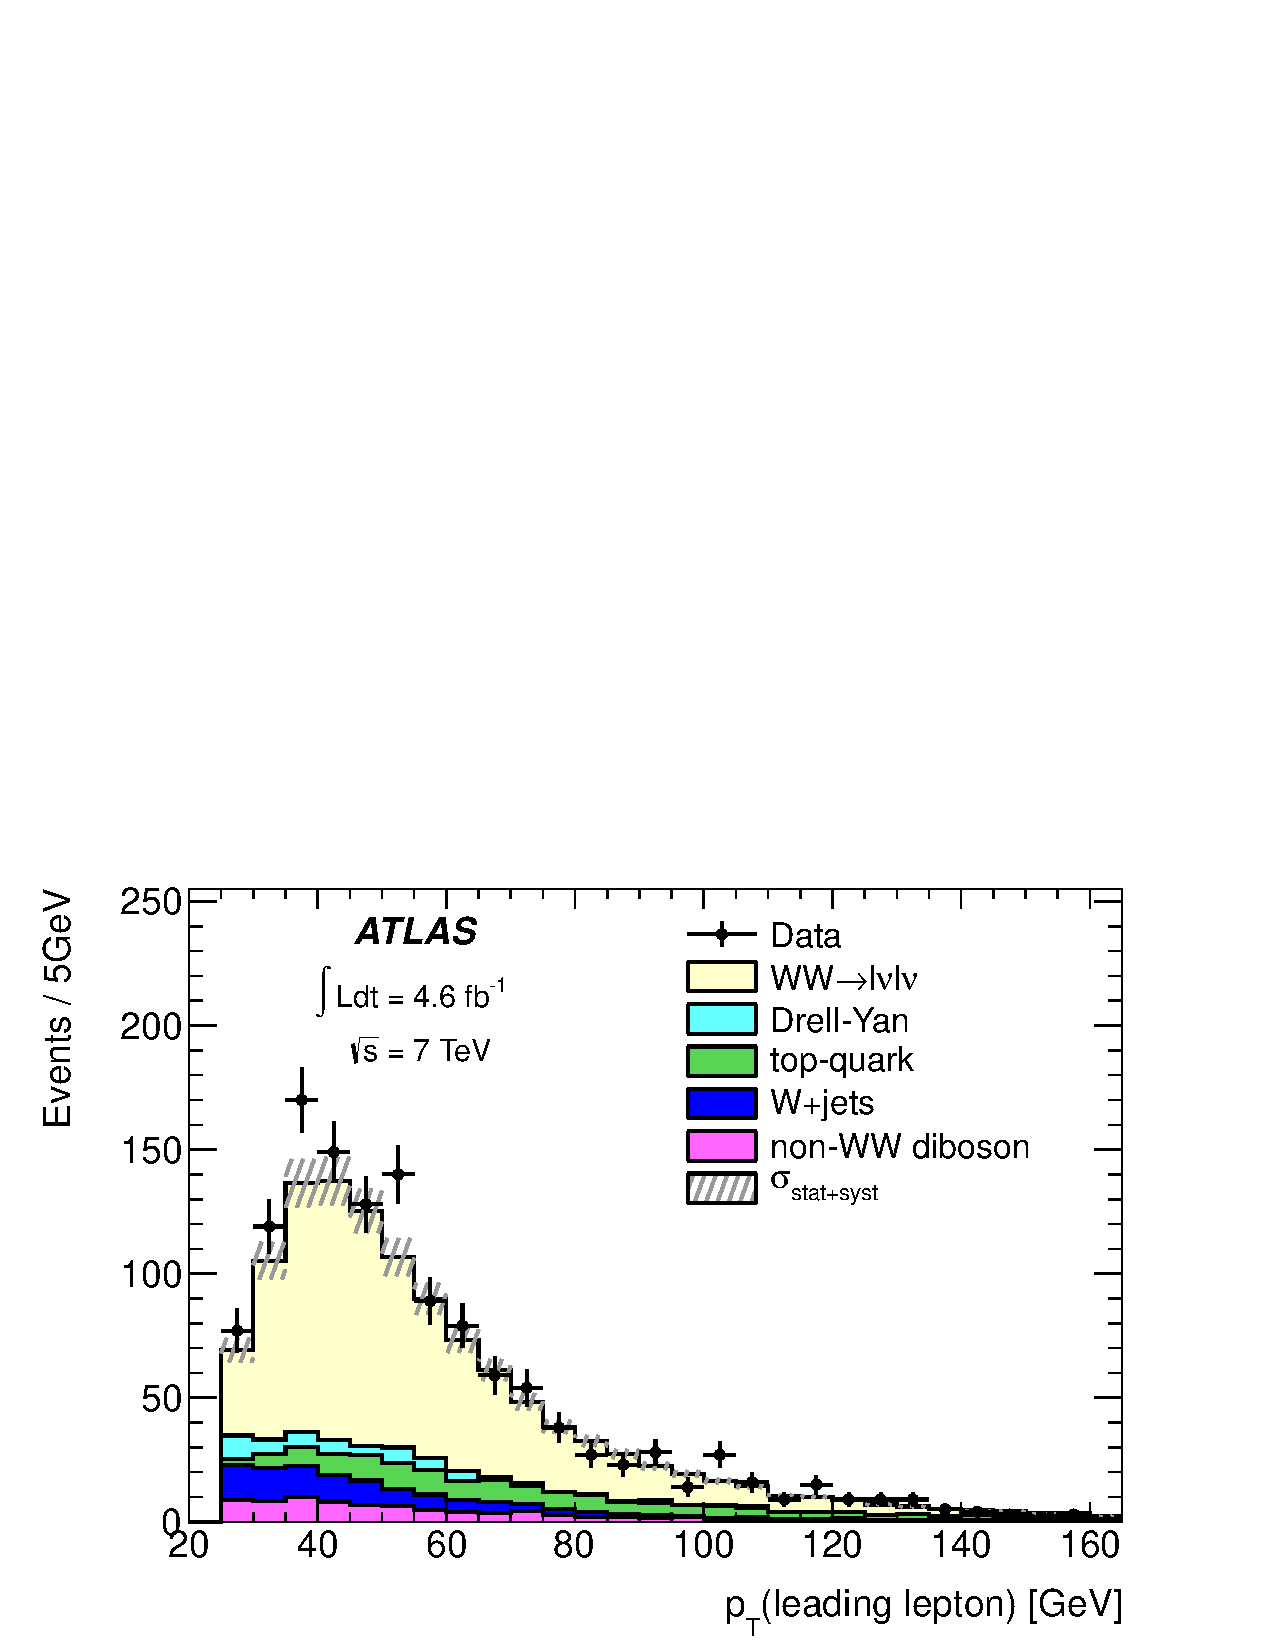
\includegraphics[width=0.495\textwidth]{tex/ww/pt_leadlep}
	\hfill
	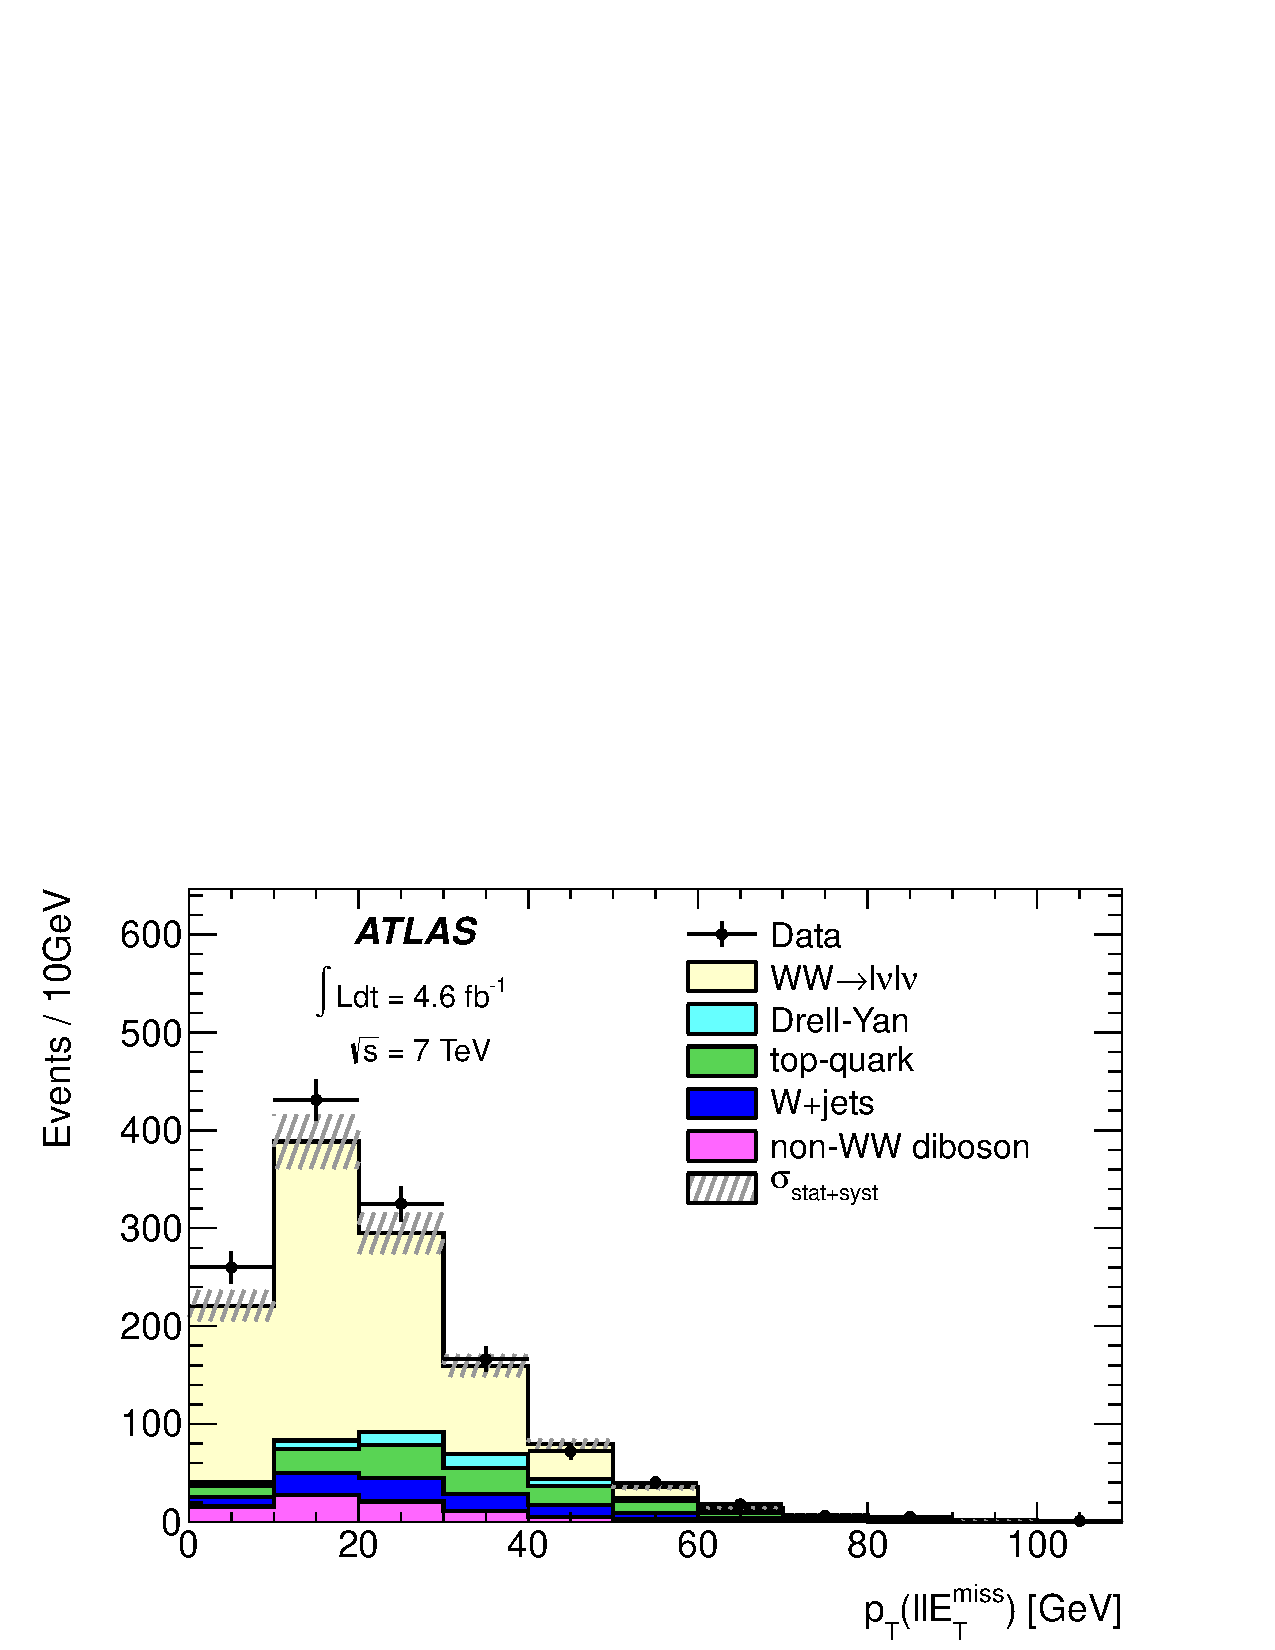
\includegraphics[width=0.495\textwidth]{tex/ww/pt_tot}
	\caption{The \pt distribution of the leading lepton (left) and the dilepton + \met 
	system (right), for all events passing the \WW event selection. Estimations of the 
	top, \Wjets and \DY (Drell-Yan) backgrounds are data-driven. The \WW signal is 
	normalised to the NLO cross section of \unit{44.7}{\pico\barn}.}
	\label{fig:ww:sr_distributions}
\end{figure}

The fiducial and total cross sections are calculated for each channel with 
(\ref{eq:ww:fid_xs}) and (\ref{eq:ww:total_xs}) respectively, using the values in 
Tables~\ref{tab:ww:cww_aww} and \ref{tab:ww:sr_yield} and an integrated luminosity of 
\unit{$L = 4.64 \pm 0.18$}{\invfb}. Systematic uncertainties in the signal acceptance and 
the total background estimation are assumed uncorrelated, and propagate to the cross 
sections via
\begin{equation}
	\parenths{\frac{\Delta\sigma^{\text{fid}}_{\WW}}{\sigma^{\text{fid}}_{\WW}}}_{\text{\!syst}}^{\!2} &= \parenths{\frac{\Delta C_{\WW}}{C_{\WW}}}^{\!2} \!+ \parenths{\frac{\Delta N_{\text{bkg}}}{N_{\text{obs}} - N_{\text{bkg}}}}^{\!2} \label{eq:ww:fid_syst} \\
	\parenths{\frac{\Delta\sigma_{\WW}}{\sigma_{\WW}}}_{\text{\!syst}}^{\!2} &= \parenths{\frac{\Delta \parenths{C_{\WW} \cdot A_{\WW}}}{C_{\WW} \cdot A_{\WW}}}^{\!2} \!+ \parenths{\frac{\Delta N_{\text{bkg}}}{N_{\text{obs}} - N_{\text{bkg}}}}^{\!2} \,. \label{eq:ww:total_syst}
\end{equation}
The relative statistical uncertainty in each channel is simply 
$\sqrt{N_{\text{obs}}} / \parenths{N_{\text{obs}} - N_{\text{bkg}}}$.

The combined total cross section from the three channels is obtained by maximising the 
likelihood function of a Poisson process
\begin{equation}
	\mathcal{L}\parenths{\sigma_{\WW} \vert N_{\text{obs}}^{\emch}, N_{\text{obs}}^{\eech}, N_{\text{obs}}^{\mmch}} &= f\parenths{N_{\text{obs}}^{\emch}; \sigma_{\WW}} \cdot f\parenths{N_{\text{obs}}^{\eech}; \sigma_{\WW}} \cdot f\parenths{N_{\text{obs}}^{\mmch}; \sigma_{\WW}} \nonumber \\
	&= \prod\limits_{i=1}^3 \frac{\eexp{-\parenths{N_{\text{sig}}^i + N_{\text{bkg}}^i}} \cdot \parenths{N_{\text{sig}}^i + N_{\text{bkg}}^i}^{N_{\text{obs}}^i}}{N_{\text{obs}}^i!}
\end{equation}
where $N_{\text{sig}}^i = \sigma_{\WW} \cdot C_{\WW}^i \cdot A_{\WW}^i \cdot \text{BR}^i 
\cdot L$ and the product over $i$ corresponds to the three channels. The best fit 
$\hat{\sigma}_{\WW}$ is that which maximises the likelihood, and the statistical 
uncertainty is obtained by finding where $\ln \mathcal{L}(\hat{\sigma}_{\WW} \pm 
\Delta\sigma_{\WW}) = \ln \mathcal{L}(\hat{\sigma}_{\WW}) - \tfrac{1}{2}$. 

The systematic uncertainty in the combined cross section is calculated with
(\ref{eq:ww:total_syst}), again using the values in Tables~\ref{tab:ww:cww_aww} and 
\ref{tab:ww:sr_yield}. The top and non-\WW diboson systematic uncertainties are 
considered correlated between all three channels. The \Wjets and \DY systematic 
uncertainties are treated as uncorrelated between the \eech and \mmch channels, though 
their combination is considered correlated with the \emch channel.

The measured cross sections are shown in \Table~\ref{tab:ww:xs_results}. The combined 
total cross section is \statsystlumi{51.9}{2.0}{3.9}{2.0}~\pico\barn, which is slightly 
higher than the theoretical prediction of \unit{$44.7\pm2.0$}{\pico\barn}. However, the 
discrepancy is not statistically significant. If contributions from \HWW and VBF \WW 
production are included, the measured cross section reduces to 
\statsystlumi{50.5}{2.0}{3.9}{2.0}~\pico\barn.

\begin{table}
	\begin{tabular}{l@{\hskip 0.25in}d{1}@{$\,\pm\,$}d{1}@{$\,\pm\,$}d{1}@{$\,\pm\,$}d{1}@{\hskip 0.2in}d{1}@{$\,\pm\,$}d{1}@{\hskip 0.3in}d{1}@{$\,\pm\,$}d{1}@{$\,\pm\,$}d{1}@{$\,\pm\,$}d{1}@{\hskip 0.2in}d{1}@{$\,\pm\,$}l}
		\toprule
		& \multicolumn{6}{c@{\hskip 0.3in}}{Fiducial cross section (\femto\barn)} & \multicolumn{6}{c}{Total cross section (\pico\barn)} \\
		& \multicolumn{4}{c@{\hskip 0.2in}}{Measured} & \multicolumn{2}{c@{\hskip 0.3in}}{Predicted} & \multicolumn{4}{c@{\hskip 0.2in}}{Measured} & \multicolumn{2}{@{}c}{Predicted} \\
		\midrule
		\emch & 262.3 & 12.3 & 20.7 & 10.2 & 231.4 & 15.7    & 51.1 & 2.4 & 4.2 & 2.0 & 44.7 & 2.0 \\
		\eech &  56.4 &  6.8 &  9.8 &  2.2 &  54.6 &  3.7    & 46.9 & 5.7 & 8.2 & 1.8 & 44.7 & 2.0 \\
		\mmch &  73.9 &  5.9 &  6.9 &  2.9 &  58.9 &  4.0    & 56.7 & 4.5 & 5.5 & 2.2 & 44.7 & 2.0 \\
		\cmidrule(lr){1-13}
		All   & \multicolumn{4}{c}{} & \multicolumn{2}{c@{\hskip 0.3in}}{} & 51.9 & 2.0 & 3.9 & 2.0 & 44.7 & 2.0 \\
		\bottomrule
	\end{tabular}
	\caption{Measured fiducial and total \WW cross sections extracted from each signal 
	region. Theoretical predictions are shown for comparison. The uncertainties in 
	measured quantities are statistical, systematic and luminosity, respectively.}
	\label{tab:ww:xs_results}
\end{table}
